\chapter{Revisão Bibliográfica}
\label{cap:revisao_bibliografica}
Neste capítulo são apresentados conceitos e pesquisas relacionados ao controle de acesso e sistemas utilizados para tal. Tópicos como Catracas e Internet das Coisas (IoT) serão igualmente retratados e discutidos neste capítulo.
\section{Referencial Teórico}

Nesta seção são expostos conceitos que reiteram a relevância da execução deste estudo no contexto da gestão de fluxo. Versando dados e informações que corroboram esta dissertação, além de outros trabalhos os quais embasam o desenvolvimento da mesma.
\subsection{Catracas}

Inseridas no cotidiano da sociedade, de forma quase desapercebida, as catracas, ou roletas, ou, do inglês, ticket gates, são utilizadas através do globo como barreiras físicas que impedem que pessoas não autorizadas acessem determinadas áreas. Estes dispositivos, assim como o ser humano, vêm sofrendo transformações e evoluindo com o passar do tempo, onde haviam outrora apenas carcaças de metal (Fig 1.), atualmente, estão inseridas tecnologias modernas que auxiliam na coleta e processamento de dados (Fig 2.).
%%%%%%%%%%%%%%%%%%%% Figure/Image No: 6 starts here %%%%%%%%%%%%%%%%%%%%

\begin{figure}[H]
	\centering
	\begin{minipage}{.5\textwidth}
	  \centering
	  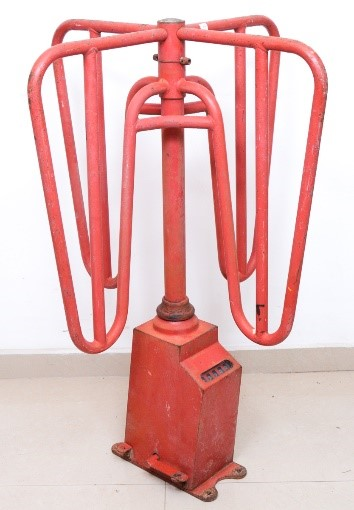
\includegraphics[width=0.95in,height=1.75in]{./media/catraca_antiga.jpg}
	  \caption{Catraca Antiga}
	  \label{fig:older}
	  \source{\cite{antiga}.}
	\end{minipage}%
	\begin{minipage}{.5\textwidth}
		\centering
		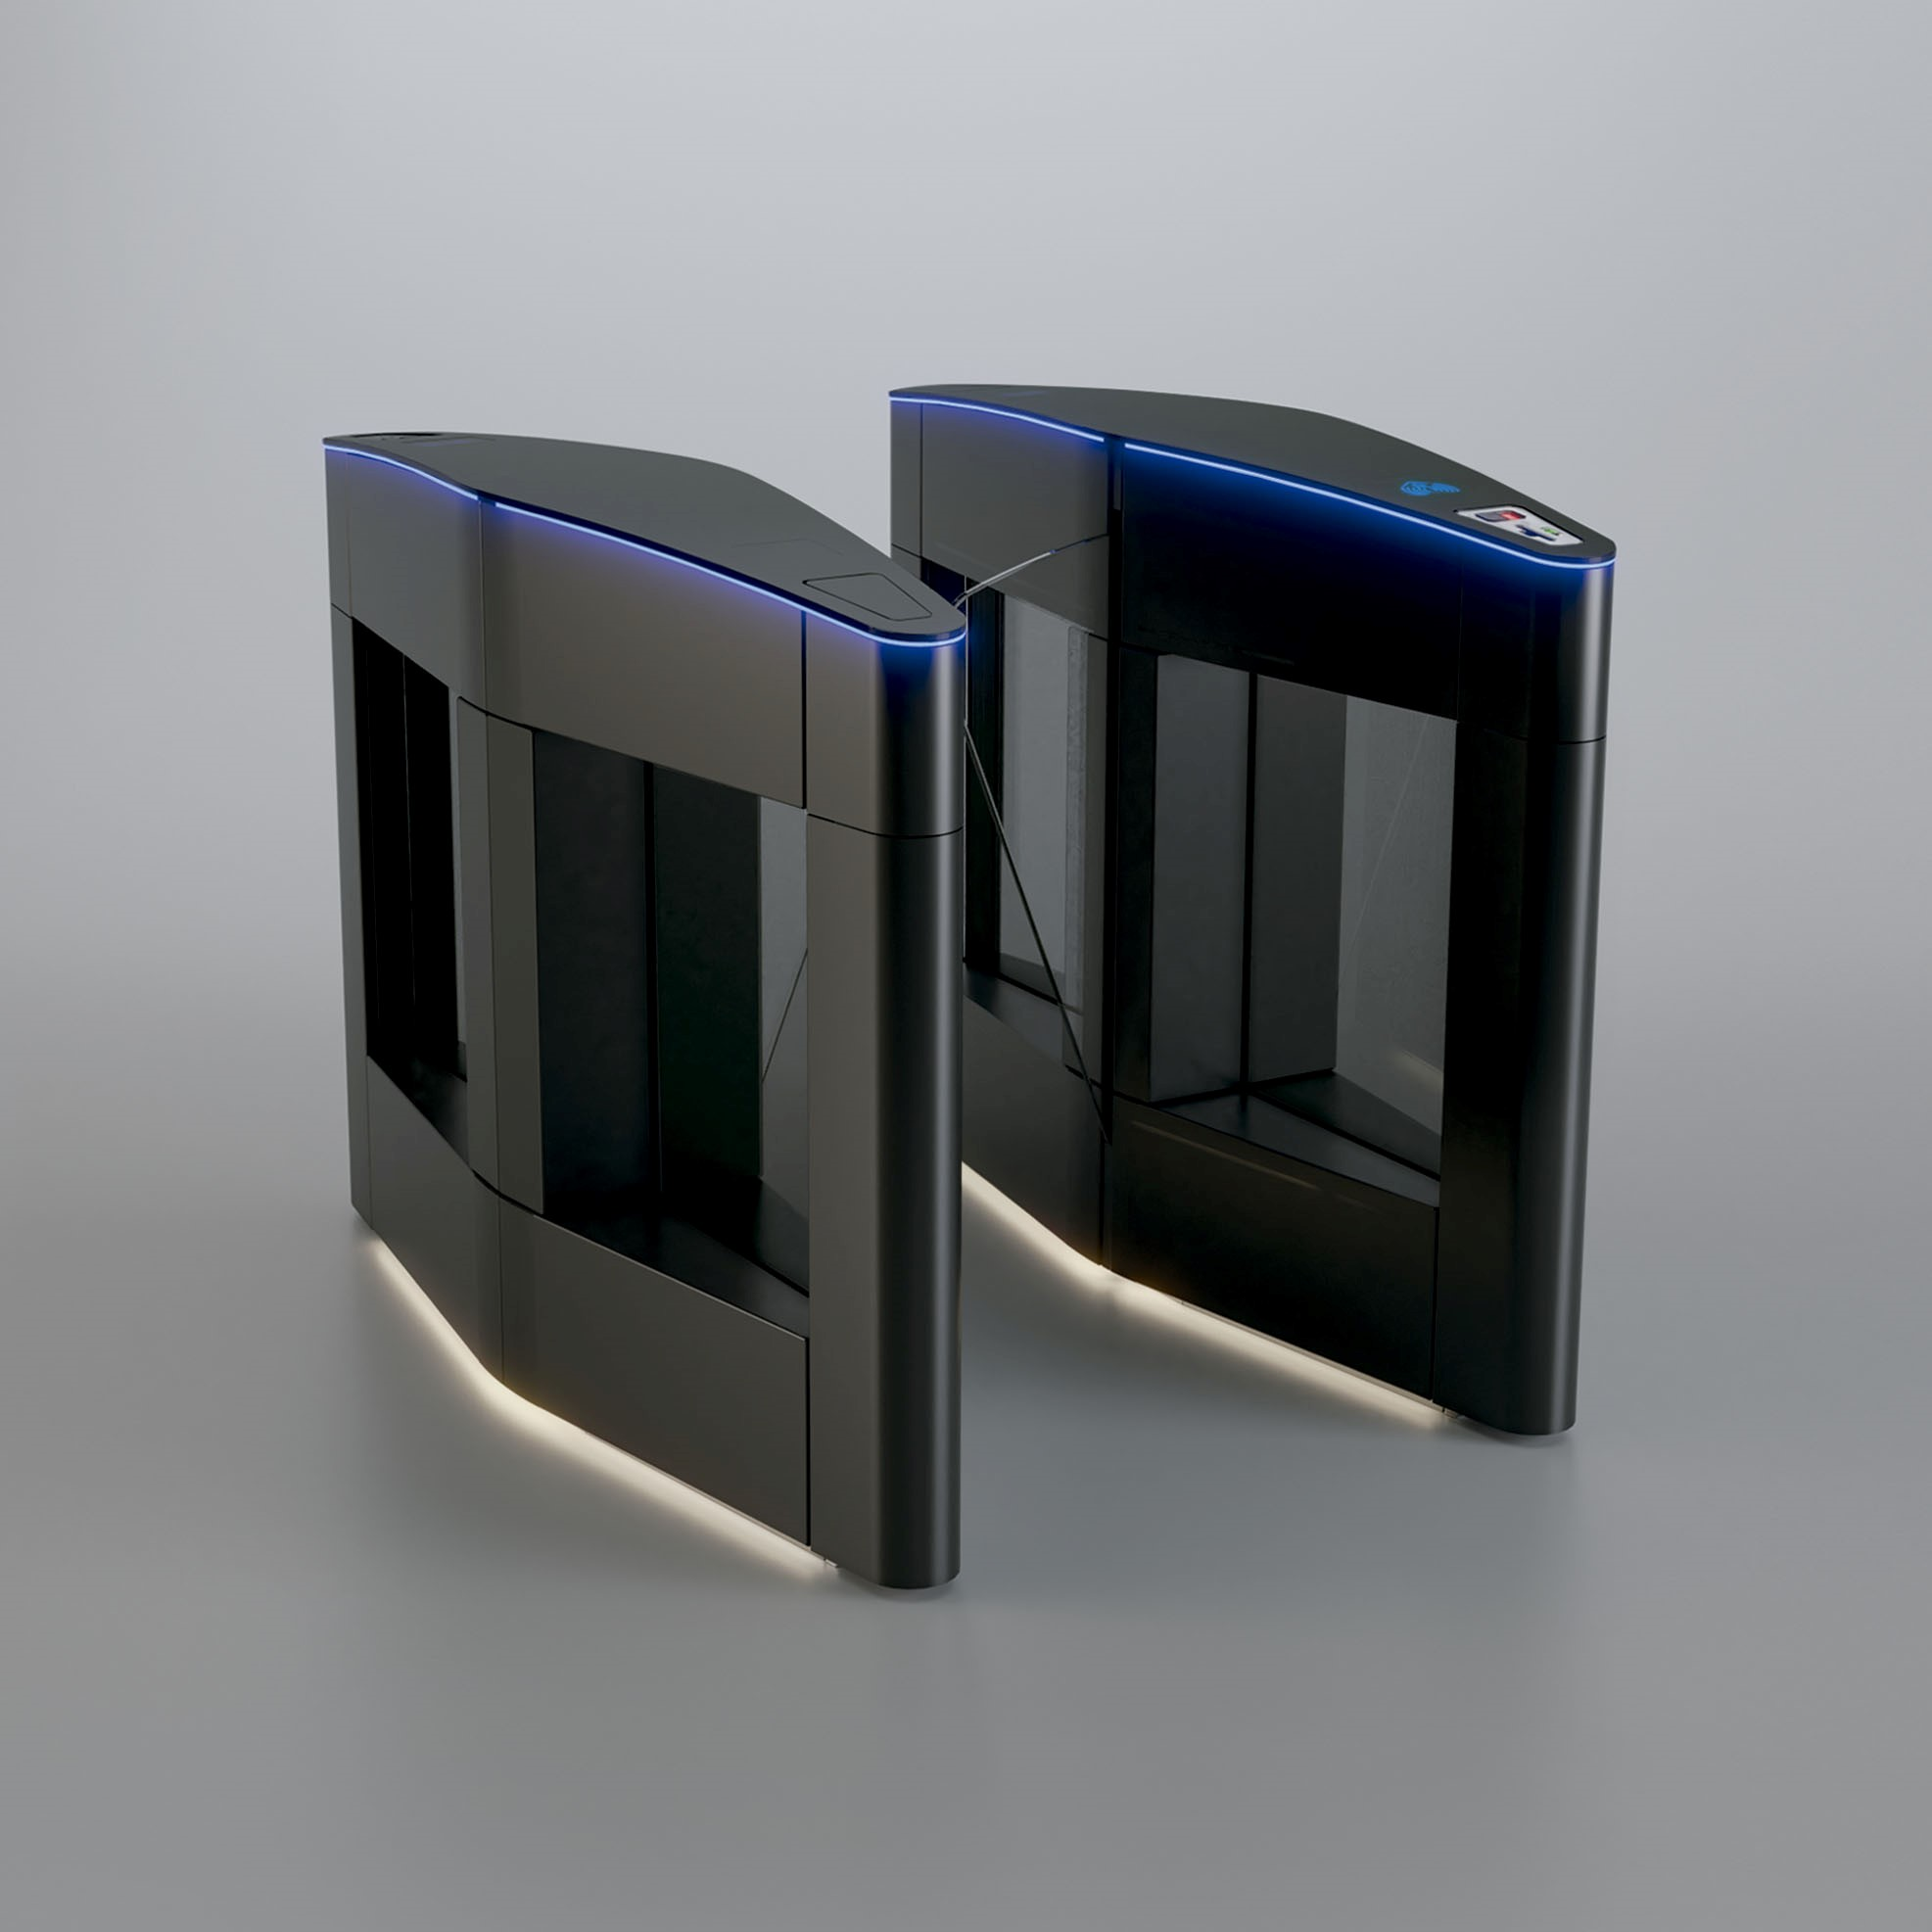
\includegraphics[width=0.95in,height=1.75in]{./media/catraca_nova.jpg}
		\caption{Catraca Nova}
		\label{fig:new}
		\source{\cite{nova}.}
	\end{minipage}
	  \end{figure}

%%%%%%%%%%%%%%%%%%%% Figure/Image No: 6 Ends here %%%%%%%%%%%%%%%%%%%%

\subsection{Internet das Coisas (IoT)}
Tendo seu primeiro uso conhecido sido feito por Kevin Auston, no que diz respeito ao termo IoT, do inglês “Internet of Things”, ou “Internet das Coisas” em tradução livre, temos a união de dois outros termos, “Internet” e “coisas”. O termo “internet” se refere a rede mundial interconectada de computadores que através do protocolo de rede TCP/IP conecta servidores e usuários em todo o globo, tendo cerca de 40\% da população mundial inserida, 7.859.533.912 de seres humanos \cite{populacao} para 4,889,155,643 de usuários \cite{usuarios}. Enquanto isso, o termo “coisas” faz referência a todo e qualquer objeto distinguível no mundo real, eletrônicos ou não, seres vivos ou não. Tendo esclarecido este ponto, não há uma única e verdadeira definição para este termo, no entanto o que a maioria dessas definições tem em comum é a ideia de que se trata de uma rede aberta e compreensível de objetos inteligentes capaz de auto-organizar e compartilhar dados, recursos e informações, reagindo e agindo de acordo com as mudanças no ambiente. Podendo ser considerada uma rede global onde a comunicação entre humanos, humanos e coisas e entre coisas pode ser feita, descrevendo um universo onde tudo pode estar interligado. \cite{iot}

\section{Trabalhos Relacionados}
Este capítulo tem como um dos seus objetivos apresentar e diferenciar os softwares e ferramentas já presentes no mercado, exemplificando suas qualidades e imprecisões e como esses contribuem para o contexto.

\subsection{Relatório Para Aquisição de Novas Catracas}
\subsubsection{Tecnibra}
A Tecnibra é uma empresa localizada no estado de Minas Gerais que utiliza software de terceiros em seus equipamentos, o mesmo permite até 4000 registros e pode trabalhar até com 4 leitores simultâneos: teclado, proximidade RFID, MIFARE, HID e leitor de impressão digital. As catracas oferecidas por essa empresa possuem garantia de 12 meses contra defeitos de fabricação. Tendo orçado em R\$ 8.560,74 cada um dos aparelhos com software de gestão para 8000 usuários.
\subsubsection{Hitech}
A Hitech é uma empresa localizada no estado do Rio de Janeiro, seus equipamentos que possuem
comunicação via RS-232, RS-485 ou TCP/IP com leitura de código de barras,
magnético ou proximidade com leitores independentes para usuário e visitantes,
pictograma orientativo e software DMP Acess II. As catracas oferecidas por essa empresa foram orçadas em R\$ 16.000,00 cada um dos aparelhos e o software de gestão em R\$ 9.000,00, além dos valores da licença do software, treinamento e contrato preventivo.
\subsubsection{Madis}
A Madis é uma empresa localizada no estado de São Paulo, seus equipamentos possuem pictogramas orientativos e direcionais com dois leitores de
proximidade Acura nas extremidades e versão biométrica que comporta 5000
funcionários utilizando somente a biometria 1:N (Só Digital) e 100.000 pessoas no
modo 1:1 (Cartão + Digital), possui capacidade de gerenciamento de até 100.000
usuários (cartões) armazenamento de até 200.000 eventos, o software oferecido é o
MD ACESSO SQL Pontos Ilimitados, No-Break inteligente para até 4 horas e a
memória para armazenamento de dados é SDCARD. As catracas oferecidas por essa empresa possuem garantia de 36 meses contra defeitos de fabricação. Tendo orçado em R\$ 16.593,00 cada um dos aparelhos e o software de gestão em R\$ 10.780,00, além do contrato de manutenção.

Como visto acima, há empresas que ofertam catracas com \textit{softwares}, próprios ou tercerizados, de diversos tipos, com diversos tipos de licenças e garantias. No entanto, o que há de semelhante entre estes produtos é o alto valor ofertado pelo conjunto mesmo que sejam tecnologias diferente, não havendo nenhuma empresa que oferte-os por um preço que, na realidade orçamentária brasileira, possa ser enxergado como baixo e os compradores não possuem qualquer flexibilização ou customização do sistema que irão receber. 

\subsection{Trabalhos Acadêmicos}
\subsubsection{Primeiro Trabalho}
O artigo "SEGURANÇA NAS INSTITUIÇÕES FEDERAIS DE ENSINO:
ESTUDO DE CASO DO IFSC ARARANGUÁ" \cite{sifeecia} apresenta a importância de aumentar a segurança no IF de Santa Catarina, unidade Araranguá, através de sistemas de controle de acesso e como o uso de tecnologia de rádio frequência (RFID) revelou-se uma possiblidade devido suas características e facilidade de uso. Se comparado a esta monografia ambas buscam objetivos semelhantes, no entanto o uso de tecnologia RFID aumenta significativamente o custo, uma vez que para a fabricação de cartões magnéticos compatíveis seria necessário uma quantidade maior de recursos, onde o valor de cada cartão RFID \cite{rfid} equivale a cerca de 5 cartões de PVC convencionais \cite{pvc}. O que fere um dos pontos chave deste trabalho, a economia.
\subsubsection{Segundo Trabalho}
A monografia "PROTÓTIPO DE CONTROLE DE ACESSO UTILIZANDO RFID PARA AUTOMATIZAÇÃO DA SEGURANÇA INTERNA DA UFERSA - CAMPUS MOSSORÓ" \cite{asiufersa} assim como o primeiro trabalho apresenta uma solução para o controle de acesso utilizando RFID. No entanto, aqui o autor mostra como utilizar a automação por meio de placas Arduino \cite{arduino}, que são placas eletrônicas capazes de interagir com o ambiente através de múltiplos sensores, utilizadas principalmente em projetos que tem como objetivo criar "objetos inteligentes" que compartilharão dados e auxiliarão no processamento de informações. Sendo relativamente similar a este projeto, tendo como falha a mesma apresentada no trabalho anterior por utilizar técnicas RFID.